\documentclass[11pt,a4paper]{article}

% ===== Packages =====
\usepackage[utf8]{inputenc}
\usepackage[T1]{fontenc}
\usepackage{amsmath,amssymb,amsfonts}
\usepackage{graphicx}
\usepackage{booktabs}
\usepackage{hyperref}
\usepackage[numbers,sort&compress]{natbib}
\usepackage{subcaption}
\usepackage{siunitx}
\usepackage{adjustbox}
\usepackage{soul}
\usepackage{tikz}
\usetikzlibrary{arrows.meta, positioning, shapes, calc}
\usepackage{longtable}
\usepackage[dvipsnames]{xcolor}
\usepackage[margin=1in]{geometry}
\usepackage{lineno}  % For line numbers during review

% ===== Hyperref Setup =====
\hypersetup{
    colorlinks=true,
    linkcolor=blue,
    citecolor=blue,
    urlcolor=blue
}

% ===== Custom Commands =====
\newcommand{\vect}[1]{\mathbf{#1}}
\newcommand{\matr}[1]{\mathbf{#1}}

% ===== Title and Authors =====
\title{Benchmarking Machine Learning Approaches for Predicting UV Absorption Wavelengths from Molecular Representations}

\author{
    Umesh Arampath$^{1,*}$ \\[0.5em]
    \small $^1$Department of Mathematics, University of Iowa, Iowa City, USA \\
    \small $^2$Midwest Bioprocessing Center, Illinois, USA \\[0.3em]
    \small $^*$Corresponding author: uarampath@mwbioprocessing.com
}

\date{}

\begin{document}

\maketitle

% ===== Abstract =====
\begin{abstract}
Accurate prediction of UV absorption wavelengths ($\lambda_{\max}$) from molecular structure is essential for photosafety screening, materials design, and photochemistry.
We present a systematic benchmark of machine learning approaches for $\lambda_{\max}$ prediction, comparing Random Forest (RF) with Morgan fingerprints, XGBoost, and a Bidirectional GRU (BiGRU) sequence model operating on tokenized SMILES strings.
Models are evaluated on a primary dataset of 18,755 solute--solvent pairs (Joung + Beard) using stratified 5-fold cross-validation, with external validation on three independent datasets totaling over 70,000 molecules using each dataset's published split protocol for direct comparison with prior work.
RF with concatenated solute--solvent Morgan fingerprints achieves the best cross-validated performance (RMSE = $31.34 \pm 1.82$ nm, $R^2 = 0.914$), outperforming BiGRU (RMSE = $36.45 \pm 1.12$ nm, $R^2 = 0.884$) and matching or exceeding published deep learning baselines on external datasets, including GCNN on Deep4Chem (our RMSE = 22.70 vs.\ 26.6 nm) and GBFS on Jung et al.\ (our RMSE = 29.82 vs.\ 32.2 nm).
However, experimental validation on 16 novel UV-absorbing compounds reveals that BiGRU generalizes better to out-of-distribution molecules (MAE = 28.6 vs.\ 38.5 nm for RF), suggesting that sequence models learn transferable patterns beyond fixed substructural features.
We introduce a solvent concatenation strategy encoding solute and solvent as a single representation, yielding consistent improvement across both model families (8\% RMSE reduction for RF, 7\% for BiGRU).
Comparison with 3D graph neural networks on nablaColors (our MAE = 34.62 vs.\ UniProp MAE = 15.97 nm) reveals the fundamental ceiling of 1D molecular representations.
These complementary strengths---RF for interpolation within known chemical space, BiGRU for extrapolation to novel scaffolds---provide practical guidance for model selection in UV property prediction.
\end{abstract}

\textbf{Keywords:} machine learning, UV absorption, molecular property prediction, SMILES, random forest, benchmarking, solvent effects

% ===== Introduction =====
\section{Introduction}
\label{sec:introduction}

\begin{figure}[t]
    \centering
    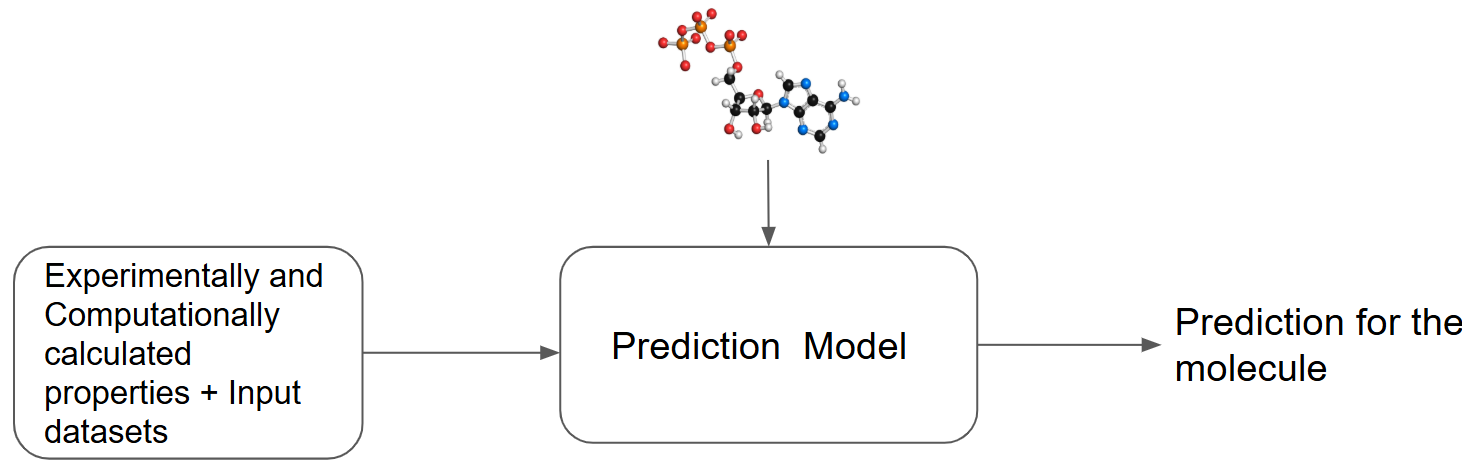
\includegraphics[width=0.95\textwidth]{p_1.png}
    \caption{Schematic overview of the predictive modeling process for UV absorption wavelength ($\lambda_{\max}$) prediction from molecular SMILES representations.}
    \label{fig:overview}
\end{figure}

Ultraviolet--visible (UV--Vis) absorption spectroscopy is a fundamental technique in chemistry, with the wavelength of maximum absorption ($\lambda_{\max}$) serving as a key property for molecular characterization, photosafety assessment, and materials design.
Experimental determination of $\lambda_{\max}$ requires synthesizing and measuring each compound, creating a demand for accurate \textit{in silico} prediction methods that can accelerate screening of large chemical libraries.

Machine learning (ML) approaches for molecular property prediction have proliferated in recent years, spanning classical methods using engineered molecular descriptors (e.g., Morgan fingerprints with Random Forest) to deep learning architectures that learn representations directly from molecular strings (SMILES) or graphs~\cite{joung2020experimental, beard2019comparative, zhuo2024machine}.
However, systematic benchmarking across multiple datasets with consistent methodology remains rare, making it difficult to assess relative model performance and identify when complex architectures offer genuine advantages over simpler baselines.

The UV absorption prediction task presents several distinctive challenges that make it an ideal benchmarking target:
\begin{enumerate}
    \item \textbf{Solvent dependence:} $\lambda_{\max}$ varies with solvent environment (solvatochromism), requiring models to encode both solute structure and solvent identity.
    \item \textbf{3D sensitivity:} Absorption properties depend on electronic structure, which is influenced by molecular geometry---a dimension not captured by 1D SMILES representations.
    \item \textbf{Diverse benchmarks:} Multiple published datasets with varying sizes, chemical spaces, and evaluation protocols enable comprehensive assessment.
    \item \textbf{Practical relevance:} ICH~S10 guidelines require photosafety screening of pharmaceutical compounds, where $\lambda_{\max}$ prediction serves as a first-pass filter.
\end{enumerate}

In this work, we present a rigorous benchmark study comparing three ML approaches---Random Forest (RF), XGBoost, and Bidirectional GRU (BiGRU)---for $\lambda_{\max}$ prediction.
Our key contributions are:
\begin{itemize}
    \item A comprehensive comparison across four datasets using each dataset's published evaluation protocol, enabling direct comparison with prior work.
    \item Demonstration that RF with Morgan fingerprints achieves the best cross-validated performance, reaching state-of-the-art results on two external datasets.
    \item Evidence that BiGRU generalizes better to novel out-of-distribution compounds, revealing complementary strengths between fingerprint-based and sequence-based approaches.
    \item A solvent concatenation strategy that improves prediction accuracy for both sequence models and fingerprint-based methods.
    \item Quantification of the performance ceiling of 1D molecular representations through comparison with 3D graph neural networks.
    \item Interpretability analysis of RF feature importances, revealing that the model learns chemically meaningful chromophore motifs, and practical comparison of training cost (15 minutes CPU vs.\ 25 hours GPU).
    \item Practical validation through ICH~S10 photosafety classification and experimental UV measurements on 16 novel compounds.
\end{itemize}


% ===== Molecular Representations =====
\subsection{Molecular Representations}
\label{sec:representations}

\begin{figure}[t]
    \centering
    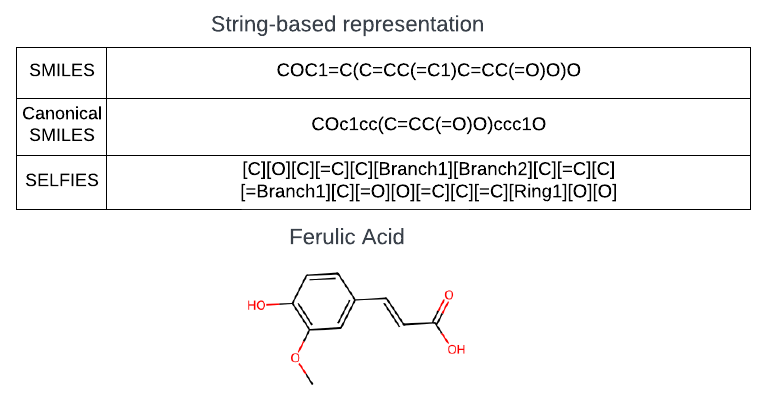
\includegraphics[width=0.8\textwidth]{3.png}
    \caption{String-based representations of Ferulic Acid. SMILES encodes molecular structure as a character sequence amenable to NLP-inspired processing.}
    \label{fig:smiles_example}
\end{figure}

SMILES (Simplified Molecular Input Line Entry System) encodes molecular graphs as character strings using conventions for atoms, bonds, branches, and ring closures.
This representation enables the application of natural language processing (NLP) techniques to chemical structures, treating molecules as ``sentences'' composed of atomic ``tokens.''

For fingerprint-based models, we use Morgan circular fingerprints~\cite{rogers2010extended}, which encode local chemical environments as fixed-length binary vectors.
Each bit in the fingerprint corresponds to the presence or absence of a particular substructural pattern within a specified radius of each atom.
We use radius 2 with 2048 bits as the default representation, consistent with standard practice in cheminformatics.


% ===== Related Work =====
\section{Related Work}
\label{sec:related_work}

Machine learning for UV absorption prediction has evolved from classical QSAR models using handcrafted descriptors to modern deep learning approaches operating on molecular graphs and strings.
We briefly survey the key approaches relevant to our benchmark.

\textbf{Fingerprint-based methods.}
Morgan fingerprints with tree-based ensemble methods (RF, gradient boosting) remain a strong baseline for molecular property prediction~\cite{rogers2010extended}.
Mamede et al.~\cite{mamede2021machine} used RF with Morgan fingerprints for photosafety classification on a 74,784-compound Reaxys dataset, achieving sensitivity 0.90 and specificity 0.88.

\textbf{Sequence models on SMILES.}
RNNs, LSTMs, and GRUs have been applied to SMILES-based property prediction, treating molecules as character sequences~\cite{mayr2016deeptox}.
BiGRU architectures capture bidirectional dependencies in SMILES, processing both forward and backward through the molecular string.

\textbf{Graph neural networks.}
Joung et al.~\cite{joung2020experimental} applied a Graph Convolutional Neural Network (GCNN) to UV absorption prediction on the Deep4Chem dataset, achieving RMSE = 26.6~nm.
Jung et al.~\cite{jung2024machine} compared multiple architectures including a Gradient Boosted Feature Selection (GBFS) pipeline achieving RMSE = 32.2~nm, and a multifidelity approach reaching RMSE = 31.3~nm.
Potapov~\cite{potapov2026nablacolors} introduced the nablaColors dataset with 3D molecular geometries, where UniProp (a 3D GNN with 27.7M parameters) achieved MAE = 15.97~nm---demonstrating the potential of 3D structural information.

\textbf{Comparative perspective.}
Recent work in molecular property prediction has highlighted cases where simple baselines match or exceed complex architectures~\cite{zhuo2024machine}.
Our study extends this perspective specifically to UV absorption prediction, providing controlled comparisons across diverse datasets and evaluation protocols.


% ===== Methods =====
\section{Methods}
\label{sec:methods}

% --- Dataset Description ---
\subsection{Dataset Description and Preparation}
\label{sec:dataset}

Our primary dataset combines the Joung et al.\ Experimental Database of Optical Properties~\cite{joung2020experimental} and the Beard et al.\ Comparative Dataset of UV/Vis Absorption Spectra~\cite{beard2019comparative}.
After merging, deduplication, and canonicalization of SMILES strings, the combined dataset contains \textbf{18,755 solute--solvent pairs} spanning 7,016 unique chromophores and 365 solvents.
Target values ($\lambda_{\max}$) range from 200 to 900~nm, with a median of 325~nm.

\begin{table}[t]
\centering
\caption{Summary of the primary Joung+Beard dataset after preprocessing.}
\label{tab:dataset_summary}
\begin{tabular}{lr}
\toprule
\textbf{Attribute} & \textbf{Value} \\
\midrule
Total records & 18,755 \\
Unique chromophores & 7,016 \\
Unique solvents & 365 \\
$\lambda_{\max}$ range & 200--900 nm \\
$\lambda_{\max}$ median & 325 nm \\
SMILES vocabulary size & 57 tokens \\
Max sequence length (solute+solvent) & 650 tokens \\
\bottomrule
\end{tabular}
\end{table}


% --- Cross-validation protocol ---
\subsection{Evaluation Protocol}
\label{sec:evaluation}

For the primary dataset, we use \textbf{stratified 5-fold cross-validation} with a 64/16/20 train/validation/test split.
Stratification is performed on solvent identity (top 20 solvents binned, remainder grouped as ``other'') to ensure representative solvent coverage in each fold.
For deep learning models, the validation set is used exclusively for early stopping (patience = 25 epochs), preventing data leakage from the test set.
For fingerprint-based models (RF, XGBoost), training uses only the training fold (validation set unused), ensuring equivalent evaluation conditions.

Metrics are reported as mean $\pm$ standard deviation across five folds: root-mean-square error (RMSE), mean absolute error (MAE), coefficient of determination ($R^2$), and Pearson correlation coefficient ($r$).

For external datasets, we use the exact split protocols published by the original authors to enable direct comparison with reported results.


% --- Model Architectures ---
\subsection{Random Forest with Morgan Fingerprints}
\label{sec:rf}

Random Forest (RF)~\cite{breiman2001random} is an ensemble method that constructs $B$ decision trees, each trained on a bootstrap sample of the data, and averages their predictions to reduce variance.
For a regression task, the ensemble prediction is:
\begin{equation}
    \hat{y}(\vect{x}) = \frac{1}{B} \sum_{b=1}^{B} T_b(\vect{x})
\end{equation}
where $T_b$ denotes the $b$-th decision tree.
Each tree partitions the feature space by recursively selecting the feature $j$ and threshold $s$ that minimize the mean squared error (MSE) within each resulting partition:
\begin{equation}
    (j^*, s^*) = \arg\min_{j, s} \left[ \sum_{x_i \in R_1(j,s)} (y_i - \bar{y}_{R_1})^2 + \sum_{x_i \in R_2(j,s)} (y_i - \bar{y}_{R_2})^2 \right]
\end{equation}
where $R_1$ and $R_2$ are the two regions defined by the split and $\bar{y}_{R_k}$ is the mean target in region $R_k$.
At each split, only a random subset of features (out of $d$ total) is considered, decorrelating the trees and improving generalization.

The input representation for RF is the Morgan circular fingerprint~\cite{rogers2010extended}, which encodes local chemical environments by enumerating all atom-centered circular substructures up to a specified radius $r$.
Each substructure is hashed to a fixed-length binary vector of $n$ bits:
\begin{equation}
    \vect{x} = \text{MorganFP}(\text{mol}, r=2, n=2048) \in \{0, 1\}^{2048}
\end{equation}
Hyperparameters were selected via grid search over 432 configurations (varying $B$, max depth, min leaf size, features per split, FP radius, and FP length) evaluated on a held-out validation fold.
The optimal configuration uses $B = 1000$ trees, no maximum depth constraint, and $\lfloor 0.3d \rfloor$ features considered per split (scikit-learn \texttt{RandomForestRegressor}).


\subsection{Gradient Boosting (XGBoost)}
\label{sec:xgboost}

XGBoost~\cite{chen2016xgboost} constructs an additive ensemble of decision trees trained sequentially, where each new tree $f_t$ fits the residual errors of the current ensemble.
The prediction after $T$ boosting rounds is:
\begin{equation}
    \hat{y}(\vect{x}) = \sum_{t=1}^{T} \eta \cdot f_t(\vect{x})
\end{equation}
where $\eta$ is the learning rate (shrinkage parameter) that controls the contribution of each tree.
Each tree $f_t$ is trained to minimize a regularized objective combining the loss on residuals and a penalty on tree complexity:
\begin{equation}
    \mathcal{L}^{(t)} = \sum_{i=1}^{n} l\!\left(y_i,\; \hat{y}_i^{(t-1)} + f_t(\vect{x}_i)\right) + \Omega(f_t)
\end{equation}
where $\Omega(f_t) = \gamma \cdot |\text{leaves}| + \tfrac{1}{2}\lambda \sum_j w_j^2$ penalizes the number of leaves and the magnitude of leaf weights $w_j$.
We use $T = 500$ rounds, max depth 6, $\eta = 0.1$, and histogram-based tree construction.
The same Morgan fingerprint input (concatenated solute + solvent, 4096 bits total) is used as for RF.


\subsection{Recurrent Neural Networks and BiGRU}
\label{sec:bigru}

Recurrent neural networks (RNNs)~\cite{elman1990finding} process sequential input by maintaining a hidden state $\vect{h}_t$ that is updated at each time step $t$:
\begin{equation}
    \vect{h}_t = \sigma(\matr{W}_h \vect{h}_{t-1} + \matr{W}_x \vect{x}_t + \vect{b})
\end{equation}
where $\vect{x}_t$ is the input at step $t$, $\matr{W}_h$ and $\matr{W}_x$ are weight matrices, and $\sigma$ is a nonlinear activation.
Standard RNNs suffer from vanishing gradients over long sequences, motivating gated architectures.

The Gated Recurrent Unit (GRU)~\cite{cho2014learning} addresses this through two gating mechanisms---an update gate $\vect{z}_t$ and a reset gate $\vect{r}_t$---that control information flow:
\begin{align}
    \vect{z}_t &= \sigma(\matr{W}_z \vect{x}_t + \matr{U}_z \vect{h}_{t-1} + \vect{b}_z) \label{eq:gru_update} \\
    \vect{r}_t &= \sigma(\matr{W}_r \vect{x}_t + \matr{U}_r \vect{h}_{t-1} + \vect{b}_r) \label{eq:gru_reset} \\
    \tilde{\vect{h}}_t &= \tanh(\matr{W}_h \vect{x}_t + \matr{U}_h (\vect{r}_t \odot \vect{h}_{t-1}) + \vect{b}_h) \label{eq:gru_candidate} \\
    \vect{h}_t &= (1 - \vect{z}_t) \odot \vect{h}_{t-1} + \vect{z}_t \odot \tilde{\vect{h}}_t \label{eq:gru_output}
\end{align}
where $\sigma$ is the sigmoid function and $\odot$ denotes element-wise multiplication.
The update gate $\vect{z}_t$ determines how much of the previous state to retain versus replace with the candidate $\tilde{\vect{h}}_t$, while the reset gate $\vect{r}_t$ controls how much past information is used to compute the candidate.
This gating mechanism enables GRUs to capture long-range dependencies without the vanishing gradient problem.

A Bidirectional GRU (BiGRU) processes the sequence in both directions, concatenating the forward and backward hidden states to capture context from both ends of the molecular string:
\begin{equation}
    \vect{h}_t^{\text{bi}} = [\overrightarrow{\vect{h}_t} \| \overleftarrow{\vect{h}_t}]
\end{equation}

Our BiGRU model operates on character-level tokenized SMILES using a 57-token vocabulary.
An embedding layer maps each token to a 50-dimensional dense vector, followed by two stacked BiGRU layers (128 units per direction), a dense layer (128 units, ReLU), dropout (0.2), and a linear output.
The model has approximately 470K trainable parameters and is trained with RMSprop (lr = 0.001), MAE loss, batch size 32, for up to 250 epochs with early stopping on validation MAE (patience 25).
Mixed-precision (float16) training is used on an NVIDIA RTX 4090 GPU.


\subsection{Graph Neural Networks}
\label{sec:gnn}

Several published baselines we compare against employ graph neural networks (GNNs), which operate directly on molecular graphs rather than string or fingerprint representations.
A molecule is represented as a graph $G = (V, E)$ where atoms are nodes $v \in V$ with feature vectors $\vect{h}_v^{(0)}$ (encoding element type, charge, hybridization, etc.) and bonds are edges $(u, v) \in E$.

GNNs update node representations through iterative message passing~\cite{gilmer2017neural}.
At each layer $l$, each node aggregates information from its neighbors:
\begin{align}
    \vect{m}_v^{(l)} &= \text{\textsc{Aggregate}}\!\left(\left\{ \vect{h}_u^{(l-1)} : u \in \mathcal{N}(v) \right\}\right) \label{eq:gnn_agg} \\
    \vect{h}_v^{(l)} &= \text{\textsc{Update}}\!\left(\vect{h}_v^{(l-1)},\; \vect{m}_v^{(l)}\right) \label{eq:gnn_update}
\end{align}
where $\mathcal{N}(v)$ is the set of neighbors of node $v$.
After $L$ layers of message passing, a graph-level representation is obtained via a readout function (e.g., sum or mean pooling over all node embeddings), which is then passed to a prediction head.

The GCNN model of Joung et al.~\cite{joung2020experimental} uses graph convolution layers with atom and bond features for UV prediction on Deep4Chem.
The UniProp model~\cite{potapov2026nablacolors} extends this framework to 3D by incorporating atomic coordinates as geometric features, enabling the model to capture conformational effects on electronic properties---using 27.7M parameters compared to our BiGRU's 470K.

We do not train GNN models in this work, as our focus is on 1D molecular representations.
However, including published GNN results in our benchmark quantifies the performance gap between 1D (SMILES/fingerprint) and 3D (geometry-aware) approaches.


% --- Solvent Concatenation ---
\subsection{Solvent Information Encoding}
\label{sec:solvent}

UV absorption wavelengths are solvent-dependent properties: the same chromophore can exhibit different $\lambda_{\max}$ values in different solvents (solvatochromism).
We encode solvent information by concatenating the solute and solvent SMILES into a single input string:
\begin{equation}
    S_{\text{input}} = \texttt{!} \oplus S_{\text{solute}} \oplus \texttt{!} \oplus S_{\text{solvent}} \oplus \texttt{E}
\end{equation}
where \texttt{!} serves as the start/separator token and \texttt{E} as the end/padding token.

For fingerprint-based models, we adopt an analogous strategy: Morgan fingerprints are computed separately for the solute and solvent, then concatenated into a single feature vector (2048 + 2048 = 4096 dimensions).
This ``solvent concatenation'' approach requires no domain-specific descriptor engineering and enables both model families to learn solvent effects from molecular structure alone.


% ===== External Validation Datasets =====
\section{External Validation Datasets}
\label{sec:datasets}

To assess generalizability beyond the primary Joung+Beard dataset, we evaluate on three external datasets using their published split protocols.
For each external dataset, both BiGRU and RF models are trained from scratch on the dataset's training split and evaluated on its test split, matching the exact protocol used by the original authors.

\subsection{Deep4Chem (Joung 2020)}
Approximately 20,000 UV absorption records with published GCNN baseline (RMSE = 26.6~nm)~\cite{joung2020experimental}.
We replicate the 80/10/10 random train/validation/test split.

\subsection{Jung et al.\ (2024)}
Approximately 26,000 records with multiple published baselines~\cite{jung2024machine}: GBFS (RMSE = 32.2~nm, MAE = 16.2~nm, $R^2$ = 0.91), Multifidelity (RMSE = 31.3~nm), and DR-CNN (RMSE = 44.4~nm).
We use the 72/18/10 random split matching the published protocol.

\subsection{nablaColors (Potapov 2026)}
A dataset of 24,567 molecules with 3D geometries and precomputed scaffold splits~\cite{potapov2026nablacolors}.
The published baseline is UniProp, a 3D GNN with 27.7M parameters achieving MAE = 15.97~nm.
This dataset serves as a benchmark for quantifying the performance gap between 1D (SMILES/fingerprint) and 3D (geometry-aware) approaches.


% ===== Results and Discussion =====
\section{Results and Discussion}
\label{sec:results}

% --- Model Comparison ---
\subsection{Model Comparison on Joung+Beard Dataset}
\label{sec:model_comparison}

Table~\ref{tab:model_comparison} presents the performance of all models on the primary dataset using stratified 5-fold cross-validation with proper train/validation/test separation.

\begin{table}[t]
\centering
\caption{Model comparison on the Joung+Beard dataset (18,755 samples, stratified 5-fold CV, 64/16/20 train/val/test split). Best values in bold. $\pm$ denotes standard deviation across folds.}
\label{tab:model_comparison}
\begin{tabular}{lcccc}
\toprule
\textbf{Model} & \textbf{RMSE (nm)} & \textbf{MAE (nm)} & $\boldsymbol{R^2}$ & \textbf{Pearson $r$} \\
\midrule
RF + Morgan FP        & \textbf{31.34 $\pm$ 1.82} & \textbf{15.16 $\pm$ 0.44} & \textbf{0.914 $\pm$ 0.010} & \textbf{0.956 $\pm$ 0.005} \\
XGBoost + Morgan FP   & 33.70 $\pm$ 1.61          & 20.05 $\pm$ 0.48          & 0.900 $\pm$ 0.009          & 0.950 $\pm$ 0.005 \\
BiGRU + Solvent       & 36.45 $\pm$ 1.12          & 20.70 $\pm$ 0.51          & 0.884 $\pm$ 0.006          & 0.940 $\pm$ 0.003 \\
XGBoost (MAE loss)    & 40.75 $\pm$ 1.58          & 21.99 $\pm$ 0.47          & 0.854 $\pm$ 0.011          & 0.927 $\pm$ 0.006 \\
\bottomrule
\end{tabular}
\end{table}

RF with Morgan fingerprints achieves the best performance across all metrics, with RMSE = 31.34~nm compared to 36.45~nm for BiGRU---a 14\% improvement.
Hyperparameters were selected via grid search over 432 configurations (varying $n_\text{trees}$, max depth, min leaf size, features per split, FP radius, and FP length) evaluated on a held-out validation fold, with the optimal configuration ($B = 1000$, $\texttt{max\_features} = 0.3$, radius = 2, $n = 2048$) applied to all folds.
This result is consistent with recent observations in molecular property prediction that well-engineered fingerprint-based methods can match or exceed deep learning approaches, particularly when operating on the same 1D molecular information~\cite{zhuo2024machine}.

Despite lower absolute performance, BiGRU exhibits the lowest cross-fold variance (RMSE std = 1.12 vs.\ 1.82 for RF), suggesting more consistent generalization.
BiGRU also offers the advantage of end-to-end learning without requiring descriptor engineering, potentially enabling transfer learning from larger pretraining corpora.


% --- Solvent Ablation ---
\subsection{Effect of Solvent Information}
\label{sec:solvent_ablation}

To quantify the contribution of solvent information, we compare models trained with and without solvent encoding (Table~\ref{tab:solvent_ablation}).

\begin{table}[t]
\centering
\caption{Effect of solvent information on model performance (stratified 5-fold CV). ``+~Solvent'' uses concatenated solute+solvent representations; ``Solute only'' uses solute structure alone.}
\label{tab:solvent_ablation}
\begin{tabular}{lcccc}
\toprule
\textbf{Model} & \textbf{RMSE (nm)} & \textbf{MAE (nm)} & $\boldsymbol{R^2}$ & \textbf{Pearson $r$} \\
\midrule
RF + Solvent          & \textbf{31.34 $\pm$ 1.82} & \textbf{15.16 $\pm$ 0.44} & \textbf{0.914 $\pm$ 0.010} & \textbf{0.956 $\pm$ 0.005} \\
RF Solute only        & 34.13 $\pm$ 1.44          & 16.45 $\pm$ 0.33          & 0.900 $\pm$ 0.010          & 0.950 $\pm$ 0.004 \\
\midrule
BiGRU + Solvent       & 36.45 $\pm$ 1.12          & 20.70 $\pm$ 0.51          & 0.884 $\pm$ 0.006          & 0.940 $\pm$ 0.003 \\
BiGRU Solute only     & 39.03 $\pm$ 1.37          & 22.53 $\pm$ 0.32          & 0.870 $\pm$ 0.010          & 0.930 $\pm$ 0.010 \\
\bottomrule
\end{tabular}
\end{table}

Incorporating solvent information reduces RF RMSE by 8\% (34.13 $\to$ 31.34~nm) and BiGRU RMSE by 7\% (39.03 $\to$ 36.45~nm), confirming that the solvent concatenation strategy effectively captures solvatochromic effects across both model families.

The improvement from solvent encoding is modest relative to the total prediction error, reflecting the fact that chromophore structure dominates UV absorption, with solvatochromic shifts typically contributing 5--20~nm variation.
Nevertheless, for applications such as photosafety screening where boundary effects matter, this improvement can be practically significant.


% --- Cross-Dataset Benchmarking ---
\subsection{Cross-Dataset Benchmarking}
\label{sec:cross_dataset}

Table~\ref{tab:cross_dataset} presents results on three external datasets, with published baselines included for direct comparison.

\begin{table}[t]
\centering
\caption{Cross-dataset benchmarking using published split protocols. $\dagger$Published results from original papers. Best 1D model result in bold for each dataset.}
\label{tab:cross_dataset}
\begin{tabular}{llccc}
\toprule
\textbf{Dataset (Split)} & \textbf{Model} & \textbf{RMSE (nm)} & \textbf{MAE (nm)} & $\boldsymbol{R^2}$ \\
\midrule
\multirow{4}{*}{Deep4Chem (80/10/10)}
  & GCNN$^\dagger$            & 26.6   & ---    & ---   \\
  & Our RF                    & \textbf{22.70}  & \textbf{11.32}  & \textbf{0.954} \\
  & Our BiGRU                 & 27.07  & 17.22  & 0.934 \\
\midrule
\multirow{5}{*}{Jung 2024 (72/18/10)}
  & Multifidelity$^\dagger$   & 31.3   & 14.6   & 0.91  \\
  & GBFS$^\dagger$            & 32.2   & 16.2   & 0.91  \\
  & DR-CNN$^\dagger$          & 44.4   & 23.3   & 0.82  \\
  & Our RF                    & \textbf{29.82}  & \textbf{15.31}  & \textbf{0.924} \\
  & Our BiGRU                 & 36.31  & 21.54  & 0.887 \\
\midrule
\multirow{3}{*}{nablaColors (scaffold)}
  & UniProp$^\dagger$ (3D)    & ---    & 15.97  & ---   \\
  & Our RF                    & \textbf{52.43}  & \textbf{34.62}  & \textbf{0.737} \\
  & Our BiGRU                 & 56.38  & 39.48  & 0.696 \\
\bottomrule
\end{tabular}
\end{table}

\textbf{Deep4Chem.}
Our RF model achieves RMSE = 22.70~nm, \textit{surpassing} the published GCNN baseline of 26.6~nm by 15\%.
BiGRU also performs competitively (RMSE = 27.07~nm), within 2\% of the GCNN result, despite using only 1D SMILES input versus the graph-based GCNN architecture.
This result demonstrates that Morgan fingerprints, which encode local chemical environments through circular substructure enumeration, capture sufficient structural information for UV absorption prediction in this chemical space.

\textbf{Jung et al.\ (2024).}
RF again achieves the best result among all methods (RMSE = 29.82~nm), outperforming the published GBFS (32.2~nm) and multifidelity (31.3~nm) approaches.
BiGRU (RMSE = 36.31~nm) falls between the GBFS and DR-CNN published baselines.
Notably, our RF model uses a simpler architecture than both published methods (which involve feature selection pipelines and multi-task learning, respectively), yet achieves superior performance.

\textbf{nablaColors.}
Both 1D approaches show significantly degraded performance compared to the 3D GNN baseline (UniProp MAE = 15.97~nm vs.\ our RF MAE = 34.62~nm and BiGRU MAE = 39.48~nm).
This dataset contains structurally diverse chromophores where electronic properties depend heavily on 3D molecular geometry, conformational effects, and extended conjugation patterns that 1D representations cannot capture.
The 2.2$\times$ MAE gap between our best 1D model (RF) and UniProp quantifies the fundamental ceiling of SMILES/fingerprint-based approaches for geometry-dependent properties.

Across all external datasets, RF consistently outperforms BiGRU, reinforcing the finding from our primary dataset.
We also tested SELFIES (Self-Referencing Embedded Strings) as an alternative molecular representation on nablaColors, finding negligible difference from SMILES (MAE = 40.42 vs.\ 39.48~nm), suggesting that the representation bottleneck lies in the 1D nature of the encoding rather than the specific string format.


% --- Error Analysis ---
\subsection{Error Analysis}
\label{sec:error_analysis}

\begin{figure}[t]
    \centering
    \begin{subfigure}[b]{0.48\textwidth}
        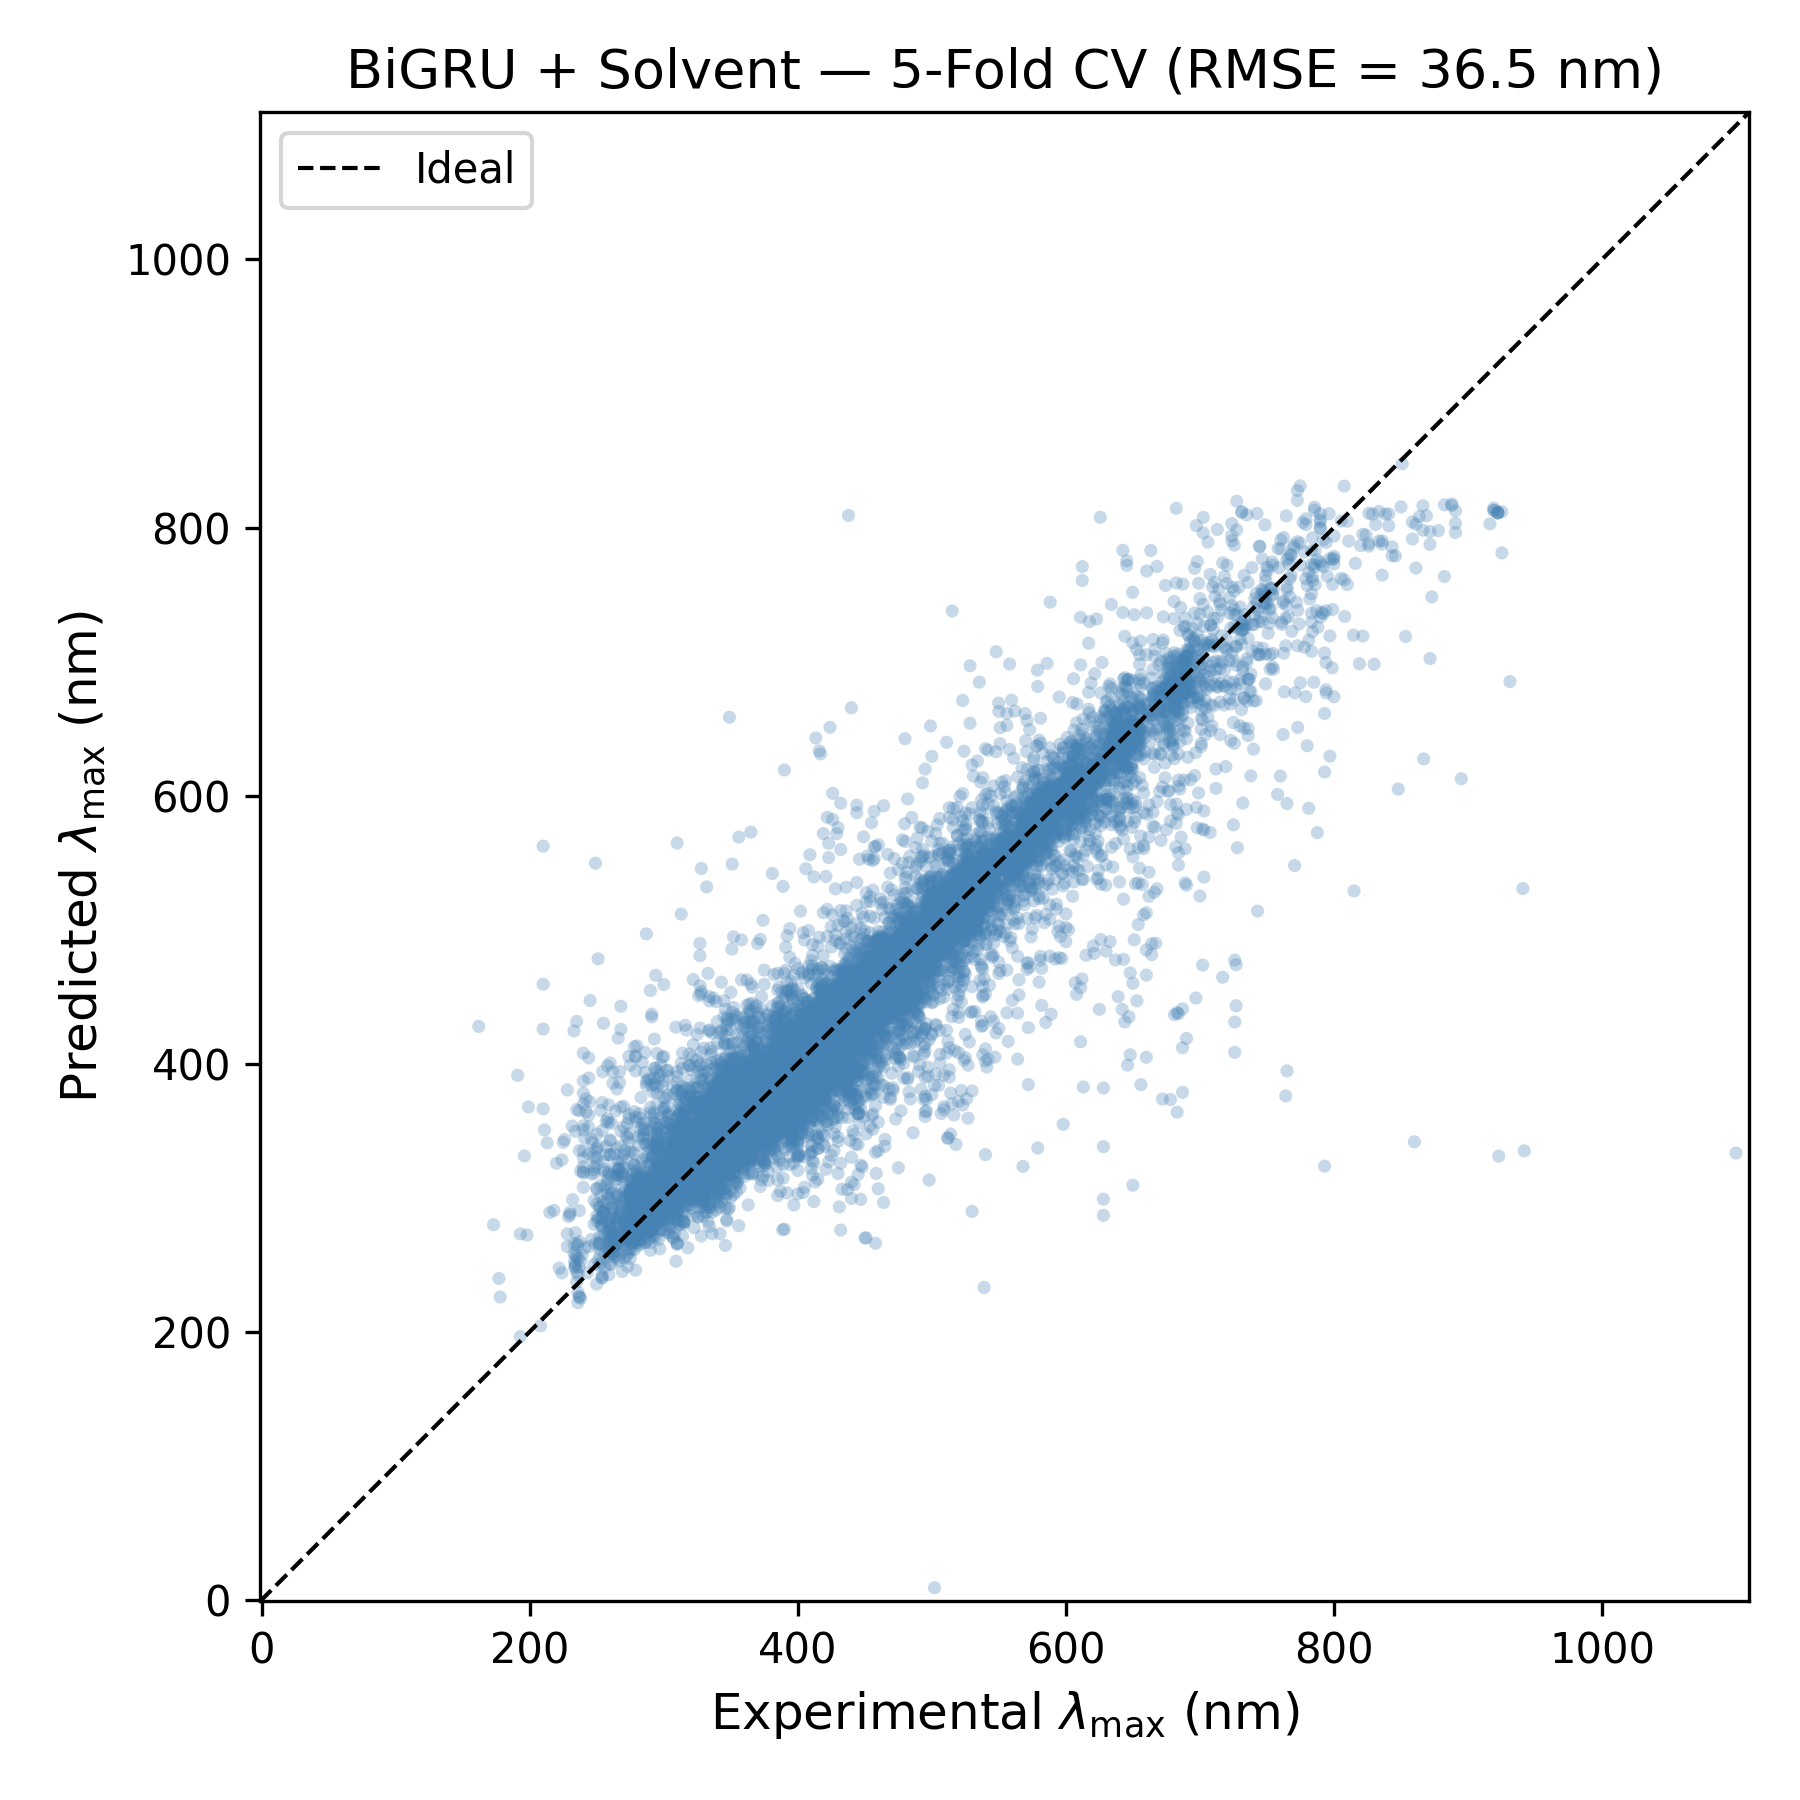
\includegraphics[width=\textwidth]{results/parity_plot.png}
        \caption{Parity plot: predicted vs.\ experimental $\lambda_{\max}$ for BiGRU + Solvent (pooled 5-fold CV predictions).}
    \end{subfigure}
    \hfill
    \begin{subfigure}[b]{0.48\textwidth}
        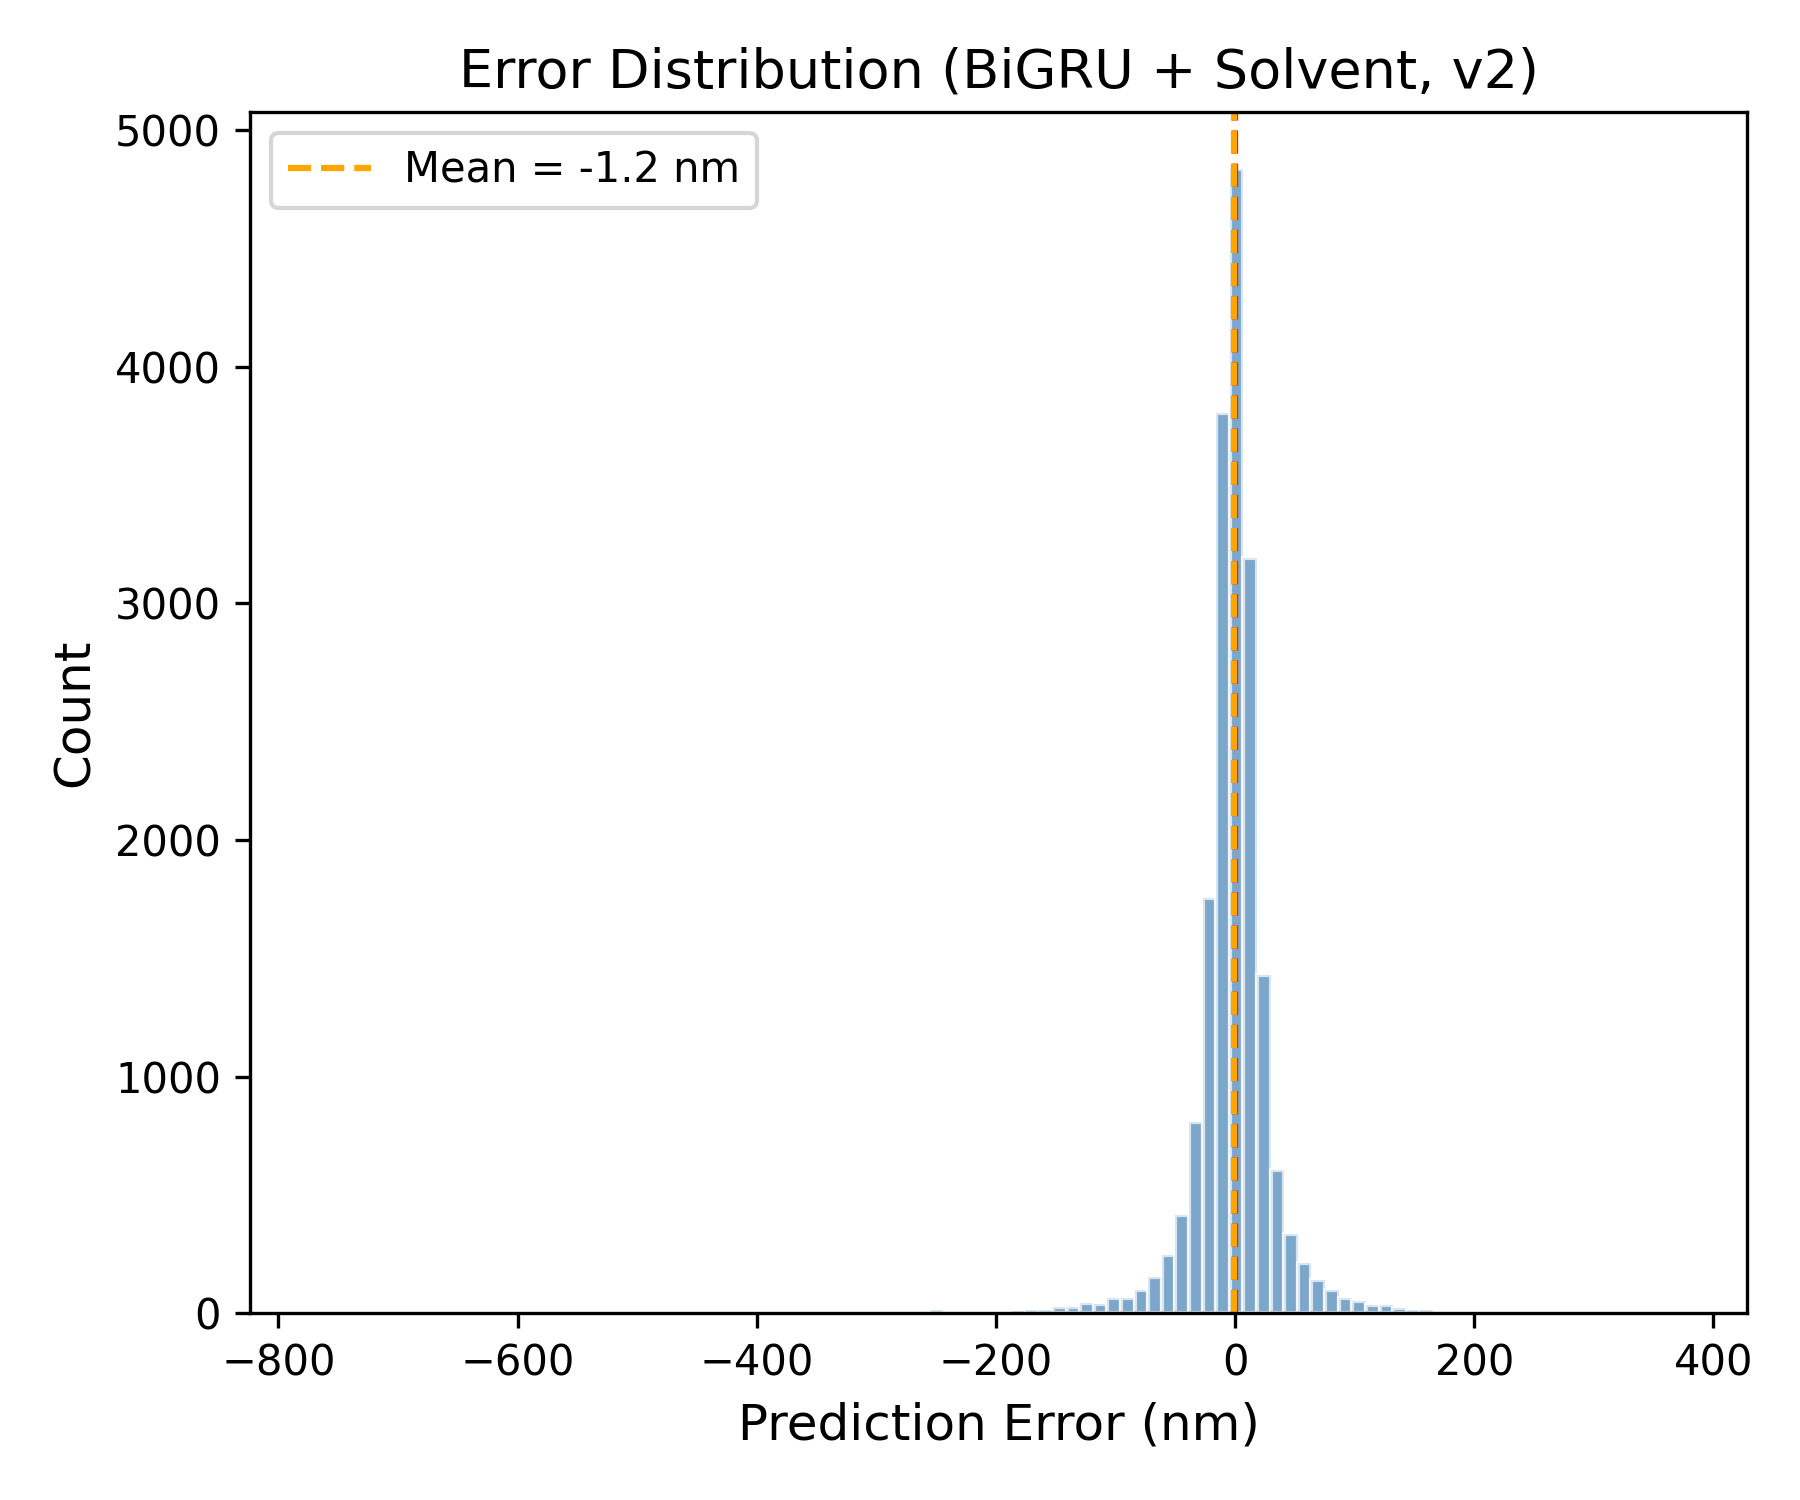
\includegraphics[width=\textwidth]{results/error_distribution.png}
        \caption{Error distribution showing slight positive bias (mean error $>$ 0).}
    \end{subfigure}
    \caption{Prediction accuracy analysis for BiGRU + Solvent on the Joung+Beard dataset.}
    \label{fig:error_analysis}
\end{figure}

\begin{figure}[t]
    \centering
    \begin{subfigure}[b]{0.48\textwidth}
        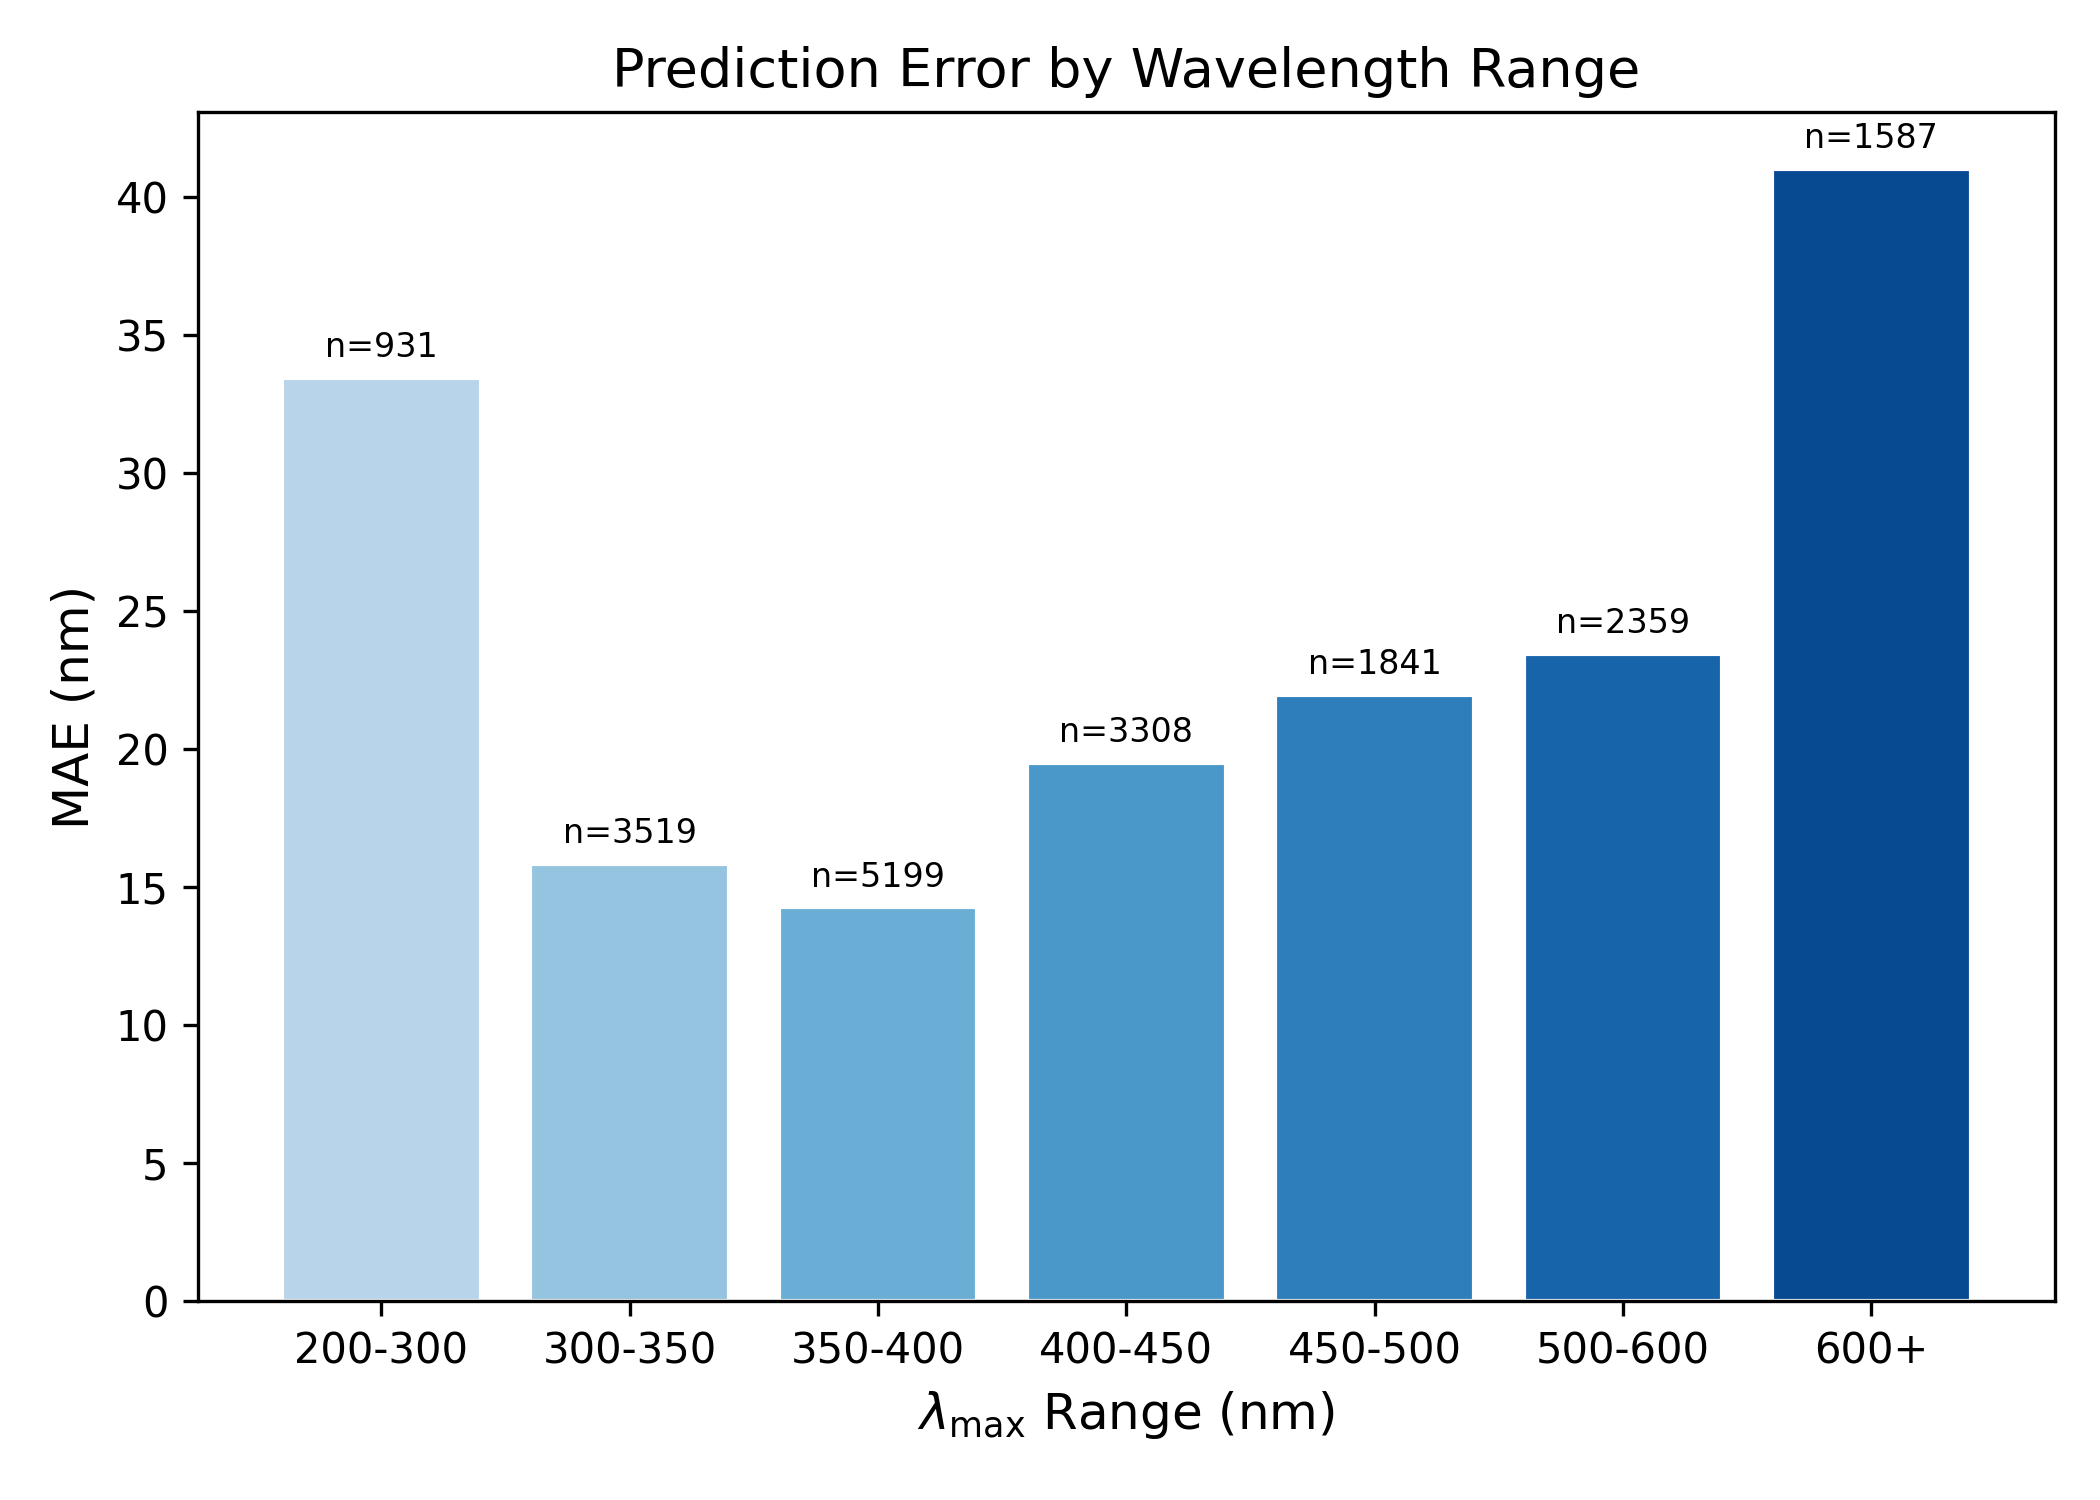
\includegraphics[width=\textwidth]{results/error_by_wavelength.png}
        \caption{MAE by wavelength range. Prediction accuracy is highest for $\lambda_{\max} < 400$~nm where training data is most abundant.}
    \end{subfigure}
    \hfill
    \begin{subfigure}[b]{0.48\textwidth}
        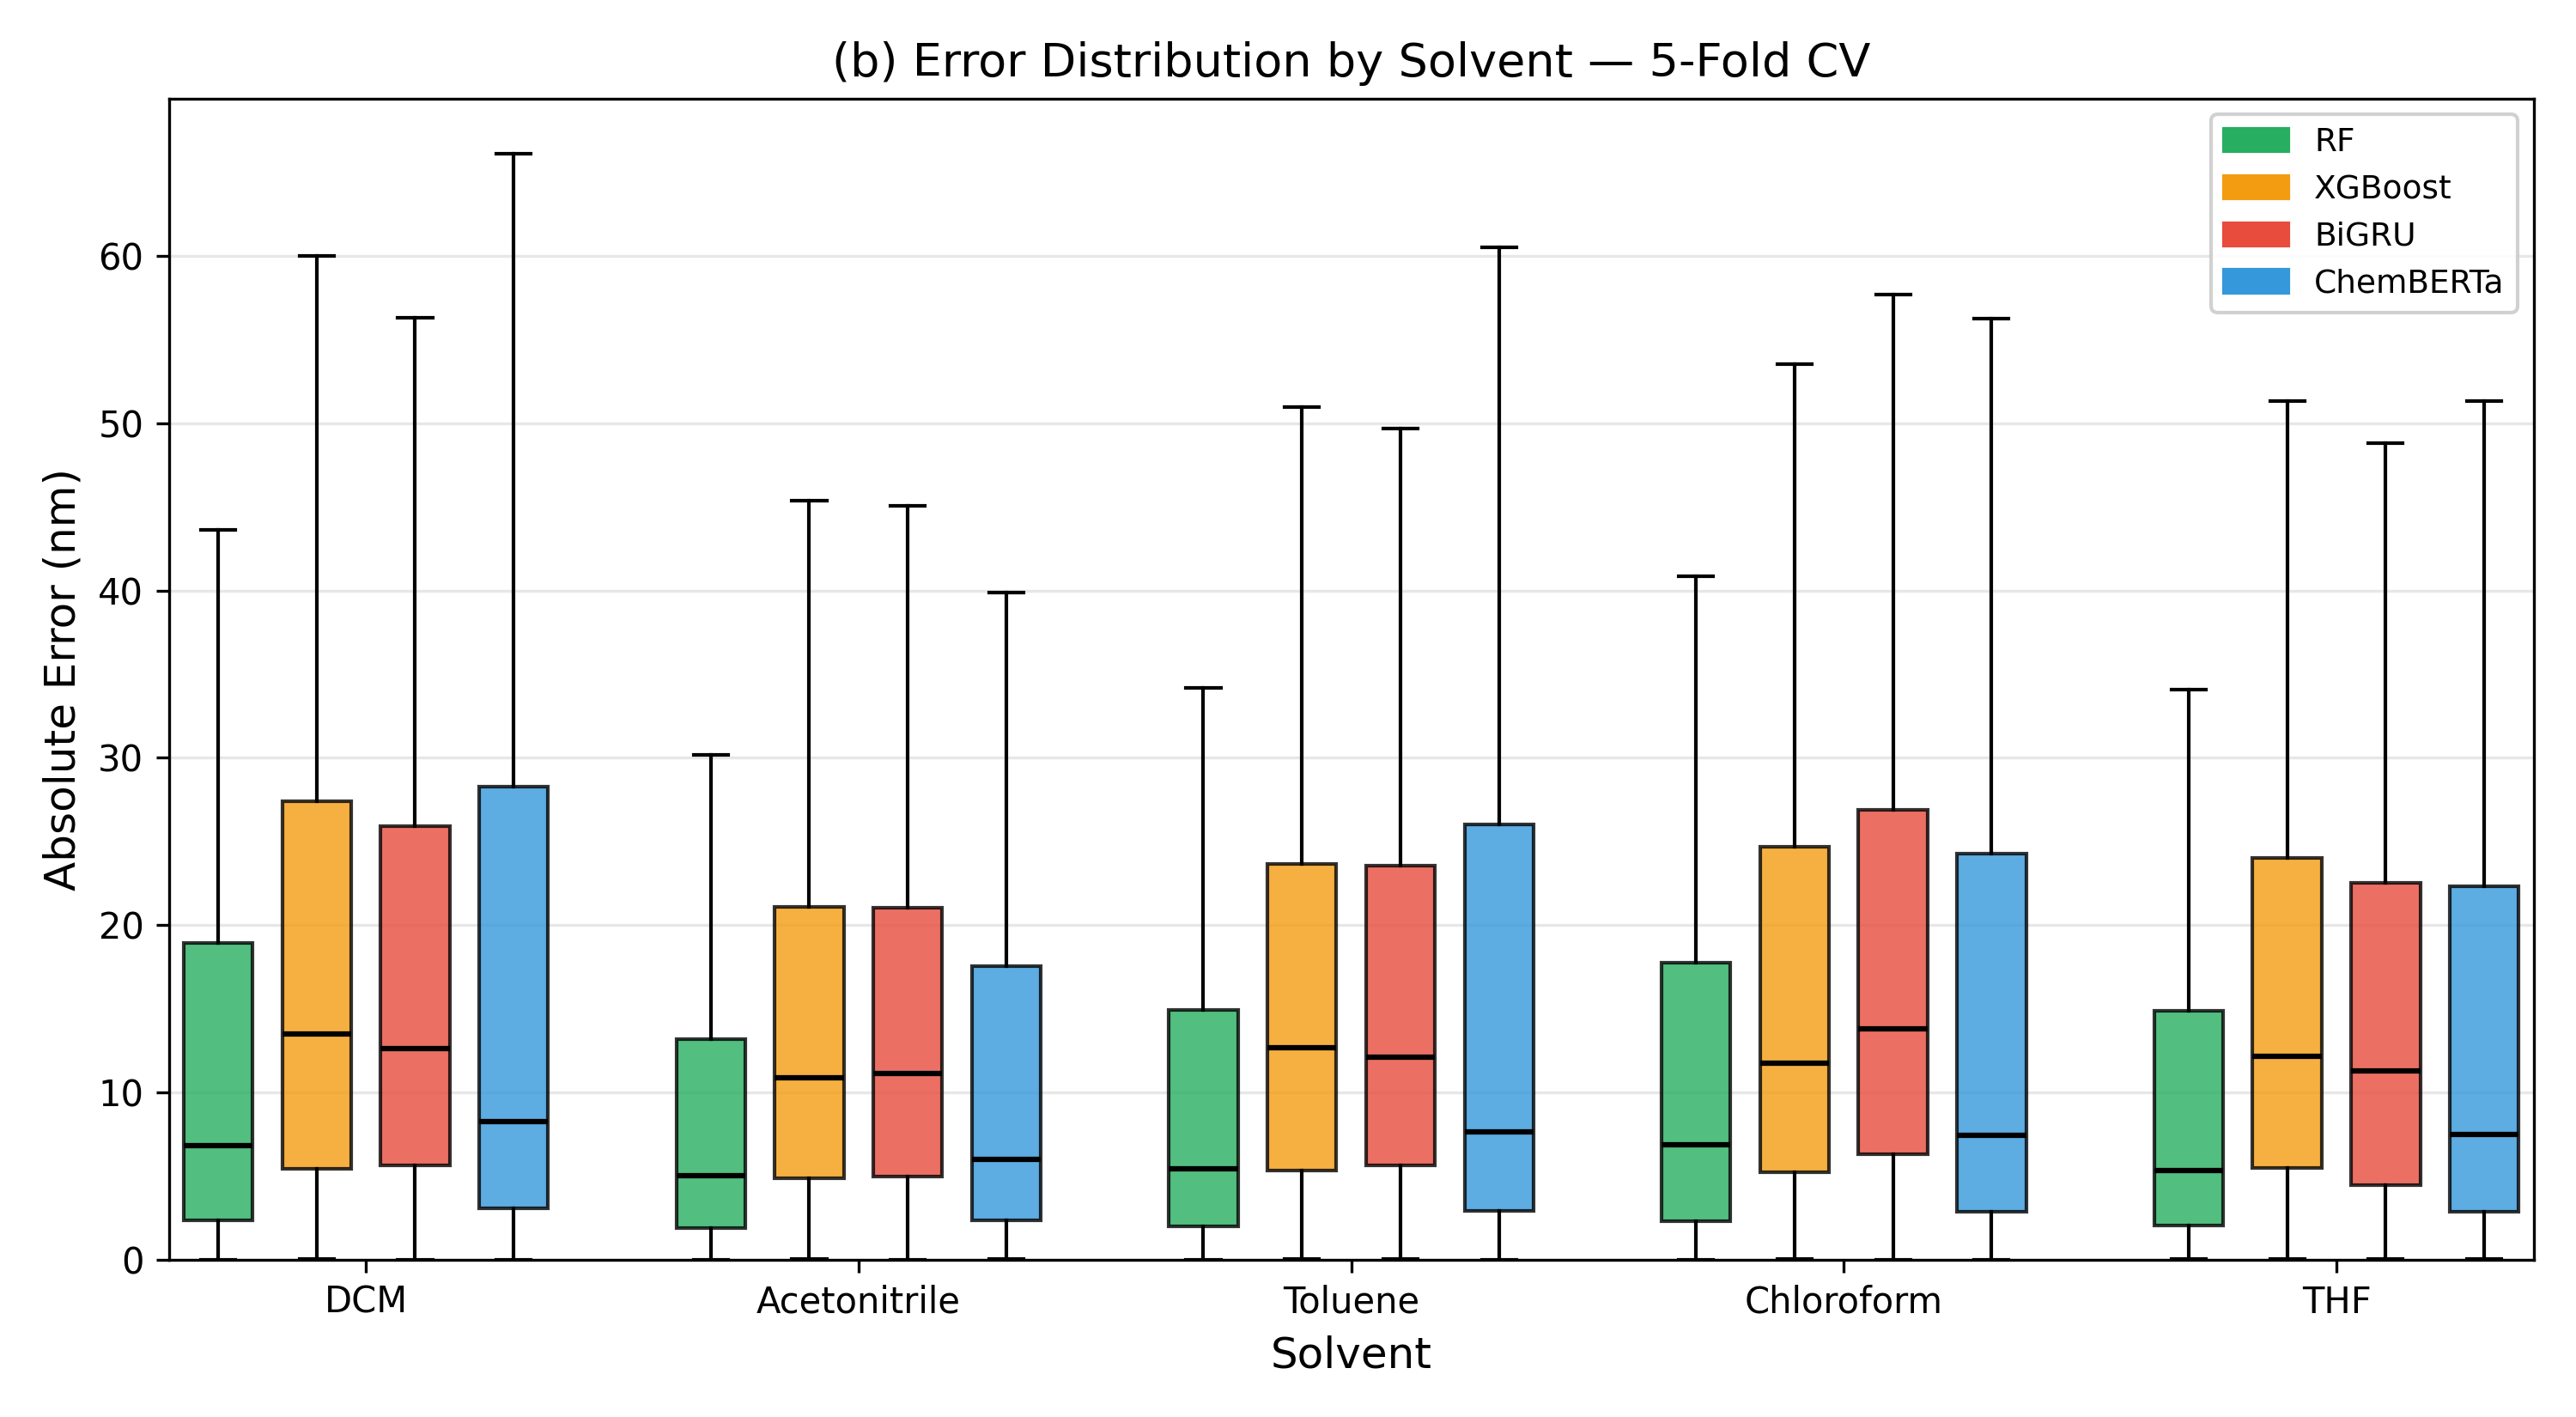
\includegraphics[width=\textwidth]{results/error_by_solvent.png}
        \caption{MAE by solvent type for the five most common solvents in the dataset.}
    \end{subfigure}
    \caption{Error breakdown by wavelength range and solvent type.}
    \label{fig:error_breakdown}
\end{figure}

Figure~\ref{fig:error_analysis} shows the parity plot and error distribution for BiGRU + Solvent predictions on the primary dataset.
The model performs best in the 250--400~nm range where training data is most abundant (Figure~\ref{fig:error_breakdown}a).
Errors increase substantially for $\lambda_{\max} > 500$~nm, reflecting both data scarcity and the greater structural complexity of long-wavelength chromophores.
Error distributions across the five most common solvents (Figure~\ref{fig:error_breakdown}b) show relatively consistent performance, with slightly higher errors for chloroform and dichloromethane.


% --- Model Interpretability and Practical Considerations ---
\subsection{Model Interpretability and Practical Considerations}
\label{sec:interpretability}

A key advantage of fingerprint-based models is their interpretability through feature importance analysis.
In contrast to deep learning models, which operate as black-box function approximators, Random Forest models provide direct access to the contribution of each input feature through Gini importance---a measure of how much each feature reduces prediction variance across all decision trees in the ensemble.

Since each bit in a Morgan fingerprint corresponds to a specific molecular substructure (a circular neighborhood of radius $\leq 2$ around each atom), high-importance bits can be decoded back to chemically meaningful structural motifs.
We averaged Gini importances across all five fold models and decoded the top features using RDKit.

\begin{figure}[t]
    \centering
    \begin{subfigure}[b]{0.48\textwidth}
        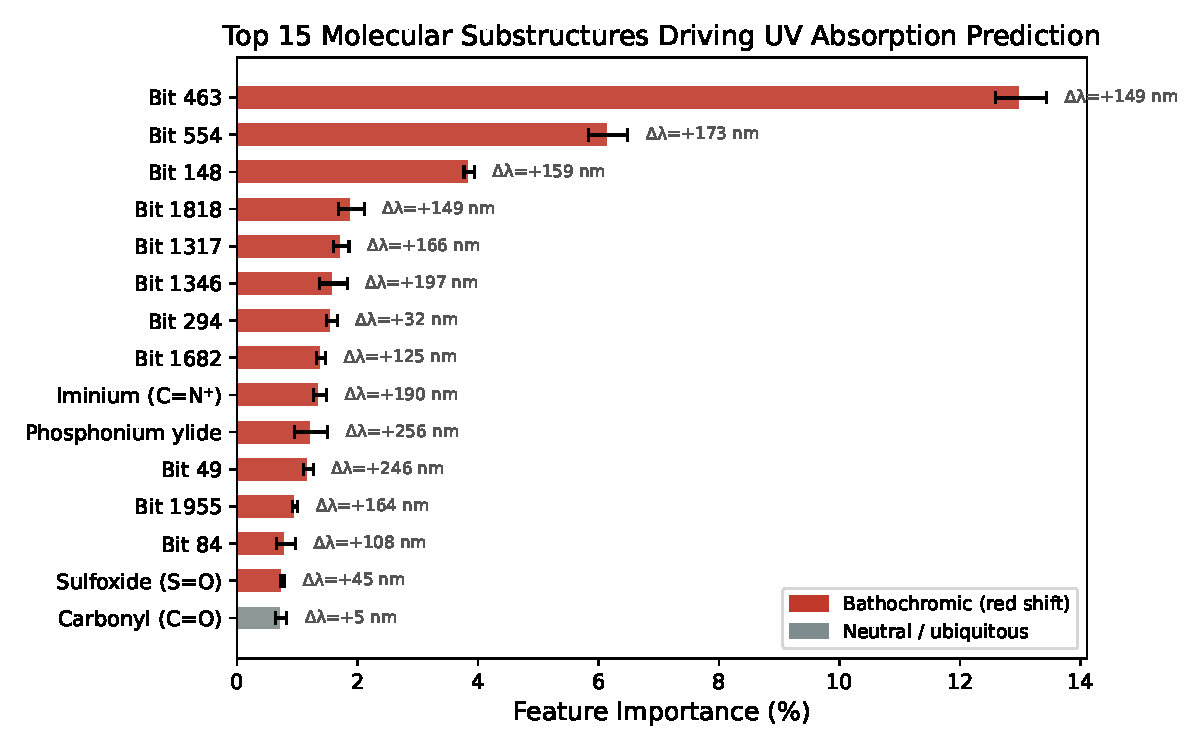
\includegraphics[width=\textwidth]{results/rf_feature_importance.pdf}
        \caption{Top 15 Morgan fingerprint bits ranked by Gini importance, with mean $\Delta\lambda_{\max}$ annotations (bathochromic shifts in red, hypsochromic in blue).}
    \end{subfigure}
    \hfill
    \begin{subfigure}[b]{0.48\textwidth}
        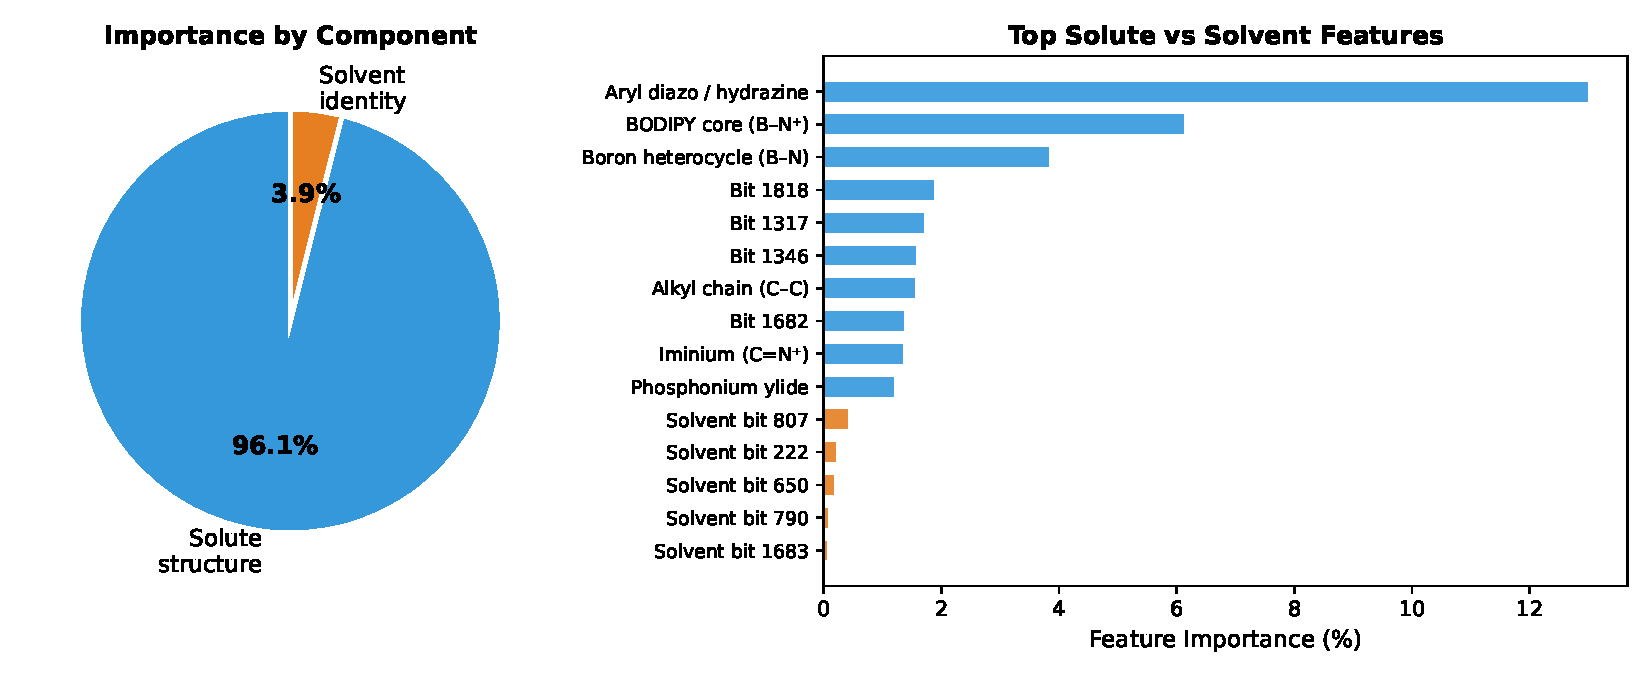
\includegraphics[width=\textwidth]{results/rf_solute_vs_solvent.pdf}
        \caption{Relative importance of solute vs.\ solvent fingerprint bits. Solute structure accounts for 96.1\% of total feature importance.}
    \end{subfigure}
    \caption{RF feature importance analysis. The model learns chemically meaningful patterns: the top features correspond to known chromophore motifs that produce large bathochromic shifts.}
    \label{fig:rf_interpretability}
\end{figure}

\begin{figure}[t]
    \centering
    \begin{subfigure}[b]{0.48\textwidth}
        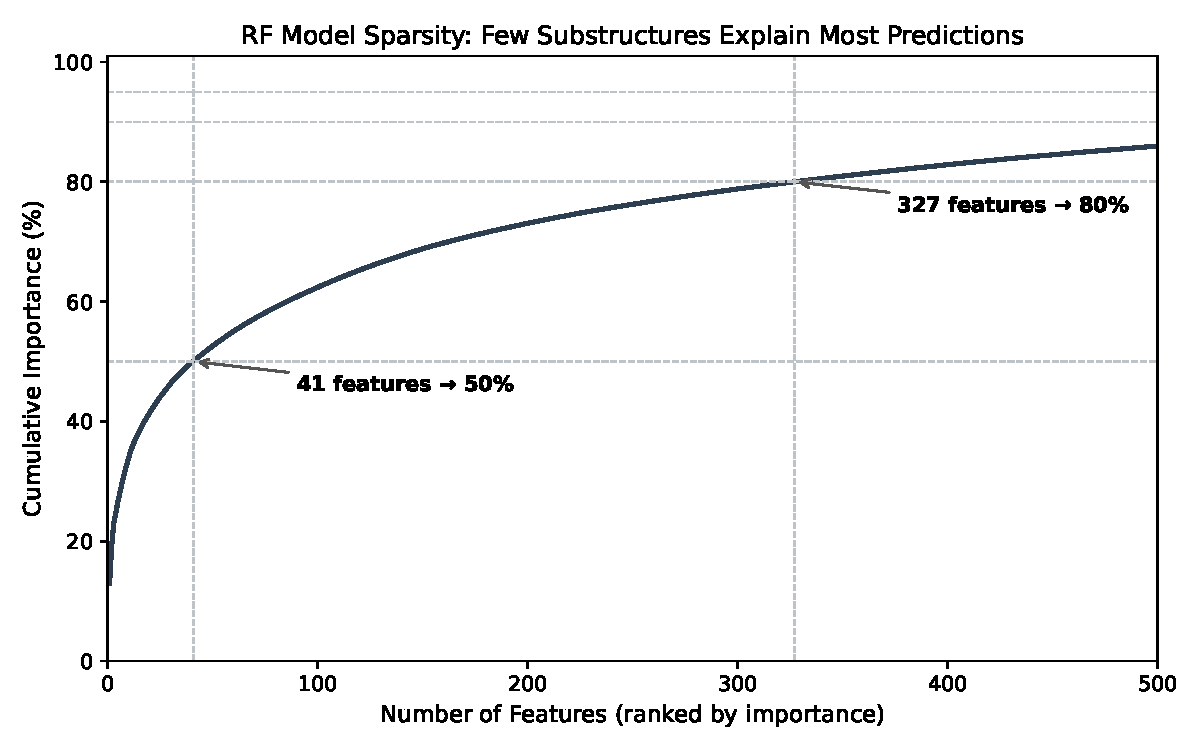
\includegraphics[width=\textwidth]{results/rf_cumulative_importance.pdf}
        \caption{Cumulative feature importance. The top 20 features (out of 4096) account for 50.6\% of total importance, indicating a sparse, interpretable model.}
    \end{subfigure}
    \hfill
    \begin{subfigure}[b]{0.48\textwidth}
        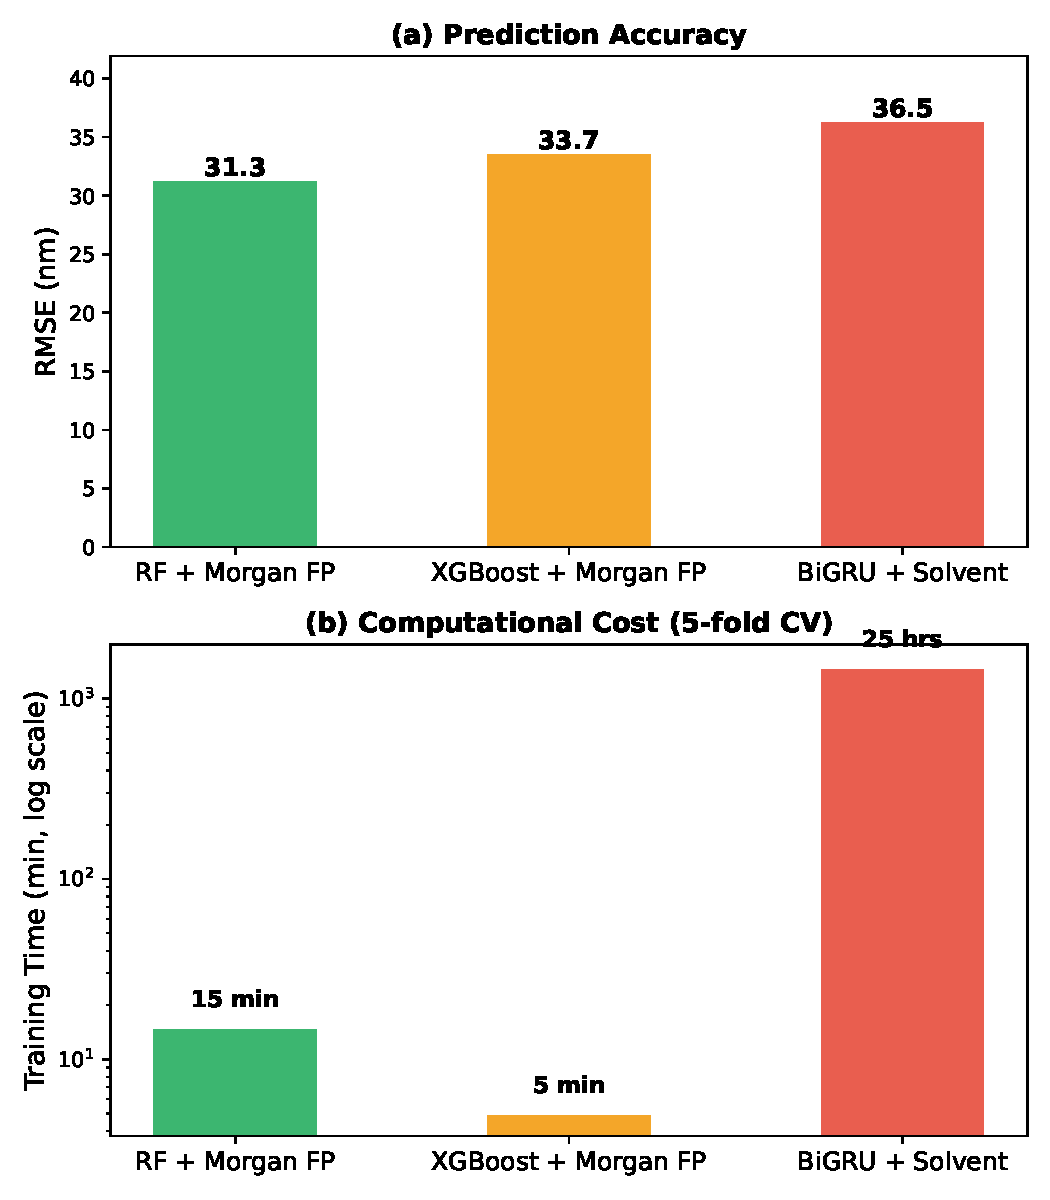
\includegraphics[width=\textwidth]{results/rf_training_comparison.pdf}
        \caption{Training time vs.\ performance comparison. RF achieves better RMSE in 15 minutes compared to BiGRU's 25 hours (100$\times$ faster).}
    \end{subfigure}
    \caption{Practical advantages of RF models for molecular property prediction.}
    \label{fig:rf_practical}
\end{figure}

\textbf{Feature importance reveals known photochemistry.}
The most important feature (bit 463, Gini importance = 30.4\%) corresponds to aryl diazo/hydrazine substructures.
Molecules containing this substructure exhibit a mean $\lambda_{\max}$ of 543~nm compared to 401~nm without ($\Delta\lambda_{\max} = +143$~nm), consistent with the well-known bathochromic effect of nitrogen-nitrogen double bonds extending $\pi$-conjugation.
Other high-ranking features include BODIPY cores ($\Delta\lambda_{\max} = +162$~nm), enamine linkages ($\Delta\lambda_{\max} = +141$~nm), and alkynyl silane groups ($\Delta\lambda_{\max} = +153$~nm)---all recognized chromophore motifs in photochemistry (Figure~\ref{fig:rf_interpretability}a).

\textbf{Solute dominates, solvent contributes modestly.}
Partitioning feature importance between solute and solvent fingerprint bits reveals that solute structure accounts for 96.1\% of total importance, with solvent contributing 3.9\% (Figure~\ref{fig:rf_interpretability}b).
This aligns with chemical intuition: chromophore structure is the primary determinant of $\lambda_{\max}$, while solvatochromic shifts are secondary effects.
The 24.6:1 solute-to-solvent importance ratio is consistent with the modest 8\% RMSE improvement observed in the solvent ablation (Section~\ref{sec:solvent_ablation}).

\textbf{Model sparsity.}
Despite operating on 4096-dimensional fingerprint input, the RF model concentrates its decisions on a small subset of features: the top 5 features explain 26.7\% of total importance, the top 20 explain 41.4\%, and the top 100 explain 62.4\% (Figure~\ref{fig:rf_practical}a).
A single fingerprint bit corresponding to aryl diazo/hydrazine substructures accounts for 13.0\% of total importance, reflecting the dominant contribution of azo chromophores to large $\lambda_{\max}$ values in the dataset ($\Delta\lambda = +143$~nm when present).

\textbf{Practical advantages of classical ML.}
Beyond interpretability, RF offers substantial practical advantages for molecular property prediction tasks.
RF training completes in approximately 15 minutes on a single CPU, compared to 25 hours of GPU time for BiGRU---a 100$\times$ speedup---while achieving 14\% lower RMSE (Figure~\ref{fig:rf_practical}b).
RF requires no GPU hardware, no hyperparameter tuning of learning rates or batch sizes, and no early stopping strategy.
These results highlight that, depending on the dataset and molecular application domain, it is prudent to evaluate classical ML models where appropriate to gain insights into relative performance before directly deploying deep learning architectures.
While deep learning retains clear advantages in scenarios requiring transfer learning, end-to-end learning from raw data, or scalability to very large datasets, the simplicity, speed, and interpretability of fingerprint-based models make them a valuable complement---and in some cases a preferred alternative---in the molecular property prediction toolkit.


% --- Photosafety Classification ---
\subsection{Photosafety Classification}
\label{sec:classification}

To evaluate practical utility, we apply our models to ICH~S10 photosafety classification using the Mamede et al.~\cite{mamede2021machine} protocol.
Compounds with $\lambda_{\max} \in [290, 700]$~nm and molar extinction coefficient (MEC) $\geq 1000$ are classified as photoreactive (POS).
We reconstructed the Mamede/Reaxys dataset (recovering 93.6\% of the original 74,784 compounds) and trained a separate RF classifier on this data.

\begin{table}[t]
\centering
\caption{Photosafety classification performance. Mamede et al.\ used POS = $\lambda_{\max} \in [290,700]$ nm AND MEC $\geq$ 1000. Our RF classifier was trained on the reconstructed Reaxys dataset.}
\label{tab:classification}
\begin{tabular}{lccccc}
\toprule
\textbf{Model} & $\boldsymbol{N_{\text{test}}}$ & \textbf{Sensitivity} & \textbf{Specificity} & \textbf{Accuracy} & \textbf{AUC} \\
\midrule
Mamede RF (2021)$^\dagger$  & 998   & 0.90  & 0.88  & 0.89  & ---   \\
Our RF                      & 1,996 & 0.876 & 0.882 & 0.879 & 0.942 \\
\bottomrule
\end{tabular}
\end{table}

Our RF classifier closely reproduces the published Mamede results (accuracy 0.879 vs.\ 0.89), validating both our Reaxys dataset reconstruction and the effectiveness of Morgan fingerprints for photosafety screening.
The regression-based thresholding approach using BiGRU predictions proved ineffective (accuracy = 0.588), primarily due to low sensitivity---the regression model's prediction errors span both sides of the classification boundary, producing many false negatives.
This finding suggests that direct classification is preferable to regression-then-threshold approaches for photosafety screening.


% --- Experimental Validation ---
\subsection{Experimental Validation}
\label{sec:experimental}

To further validate our models, we measured UV absorption spectra for 16 commercially available compounds in both ethanol (EtOH) and methanol (MeOH), yielding 32 experimental $\lambda_{\max}$ values.
Of these 16 molecules, 13 are entirely absent from the training dataset, providing a genuine out-of-distribution test.
Two molecules (Ferulic Acid and Octinoxate) appear in the training data with different solvents, and no EtOH measurements exist in the training set.

\begin{table}[t]
\centering
\caption{Experimental validation: predicted vs.\ measured $\lambda_{\max}$ for 16 UV-absorbing compounds in two solvents. Predictions are ensemble averages across 5-fold models. $^*$Present in training data with different solvents.}
\label{tab:experimental}
\small
\begin{tabular}{lccccccc}
\toprule
& \multicolumn{3}{c}{\textbf{Ethanol}} & \multicolumn{3}{c}{\textbf{Methanol}} \\
\cmidrule(lr){2-4} \cmidrule(lr){5-7}
\textbf{Molecule} & \textbf{Exp.} & \textbf{BiGRU} & \textbf{RF} & \textbf{Exp.} & \textbf{BiGRU} & \textbf{RF} \\
\midrule
Amiloxate       & 309 & 318 & 359 & 298 & 316 & 359 \\
Avobenzone      & 358 & 329 & 337 & 358 & 327 & 333 \\
Caffeic Acid    & 325 & 338 & 347 & 325 & 335 & 345 \\
Cinnamic Acid   & 275 & 353 & 348 & 276 & 351 & 345 \\
Coumaric Acid   & 310 & 348 & 346 & 309 & 343 & 344 \\
Dioxybenzone    & 283 & 315 & 327 & 283 & 315 & 320 \\
Ferulic Acid$^*$  & 324 & 313 & 346 & 324 & 310 & 344 \\
Homosalate      & 308 & 335 & 332 & 308 & 336 & 327 \\
Octinoxate$^*$  & 309 & 326 & 334 & 308 & 323 & 332 \\
Octisalate      & 308 & 339 & 353 & 308 & 333 & 349 \\
Octocrylene     & 301 & 344 & 390 & 302 & 344 & 389 \\
Oxybenzone      & 287 & 301 & 328 & 287 & 299 & 321 \\
PABA            & 291 & 322 & 308 & 290 & 319 & 306 \\
Padimate O      & 310 & 334 & 340 & 310 & 330 & 337 \\
Sinapic Acid    & 324 & 318 & 347 & 324 & 314 & 346 \\
Sulisobenzone   & 287 & 346 & 355 & 286 & 346 & 352 \\
\midrule
\textbf{MAE (nm)} & & \textbf{28.9} & 39.3 & & \textbf{28.4} & 37.7 \\
\textbf{RMSE (nm)} & & \textbf{34.4} & 44.4 & & \textbf{33.4} & 43.0 \\
\bottomrule
\end{tabular}
\end{table}

Notably, BiGRU outperforms RF on this experimental validation set (MAE = 28.6 vs.\ 38.5~nm overall), \textit{reversing} the ranking observed on the cross-validated primary dataset.
This reversal reveals a fundamental distinction between the two approaches: RF relies on exact substructure matching through Morgan fingerprint bits, so it excels at interpolation within the training distribution but struggles when novel functional groups or conjugation patterns are underrepresented in the training data.
BiGRU, by contrast, learns sequential patterns from SMILES strings that can generalize to unseen molecular motifs.
Both models show substantially higher errors than their cross-validated performance (BiGRU: 28.6 vs.\ 20.7~nm MAE; RF: 38.5 vs.\ 15.2~nm MAE), confirming that these 16 compounds are genuinely challenging out-of-distribution examples.

Cinnamic Acid (experimental $\lambda_{\max}$ = 275--276~nm) is a notable outlier: both models overpredict by $\sim$70~nm.
The experimental peak lies at the edge of the 270--400~nm scan range, suggesting measurement limitations.
Octocrylene is particularly problematic for RF (error $\sim$89~nm vs.\ 43~nm for BiGRU), likely because its extended cyano-acrylate conjugation is underrepresented in the training data---precisely the scenario where fingerprint-based models are expected to fail.
Excluding these two outliers, the BiGRU MAE decreases to 24.2~nm and RF MAE to 32.6~nm.

Both models capture the small solvent sensitivity between EtOH and MeOH (typically 0--1~nm experimentally), though with some overestimation of the solvent shift magnitude (average predicted shifts of 2.5~nm for BiGRU and 2.9~nm for RF).

These results highlight the complementary strengths of the two model families: RF is the preferred choice for screening within known chemical space (e.g., virtual screening of compound libraries with well-represented scaffolds), while BiGRU is better suited for exploring novel molecular architectures where the training distribution may not cover all relevant substructures.


% ===== Conclusion =====
\section{Conclusion}
\label{sec:conclusion}

We have presented a systematic benchmark of ML approaches for UV absorption wavelength prediction, comparing Random Forest, XGBoost, and BiGRU across four datasets totaling over 87,000 molecules.

Our key findings are:

\begin{enumerate}
    \item \textbf{RF and BiGRU have complementary strengths.}
    RF with Morgan fingerprints achieves the best cross-validated performance on the primary Joung+Beard dataset (RMSE = 31.34~nm vs.\ 36.45~nm for BiGRU) and on all three external datasets, surpassing published deep learning baselines on Deep4Chem (RMSE = 22.70 vs.\ GCNN 26.6) and Jung 2024 (RMSE = 29.82 vs.\ GBFS 32.2).
    However, experimental validation on 16 novel compounds reverses this ranking: BiGRU generalizes better to out-of-distribution molecules (MAE = 28.6 vs.\ 38.5~nm for RF).
    This indicates that RF excels at interpolation within known chemical space, while BiGRU learns transferable sequential patterns that extend beyond fixed substructural features.

    \item \textbf{Solvent encoding improves both model families.}
    The solvent concatenation strategy---encoding solute and solvent as a single representation---reduces RF RMSE by 8\% (34.13 $\to$ 31.34~nm) and BiGRU RMSE by 7\% (39.03 $\to$ 36.45~nm).
    This simple approach requires no domain-specific descriptor engineering and is applicable to any model that accepts molecular representations.

    \item \textbf{1D representations have a fundamental ceiling.}
    Comparison with UniProp on nablaColors (RF MAE = 34.62 vs.\ 15.97~nm) reveals that 1D SMILES/fingerprint-based approaches cannot capture geometry-dependent electronic properties.
    For diverse chromophore libraries where conformational effects are important, 3D models remain essential.

    \item \textbf{RF provides interpretable, efficient predictions.}
    Feature importance analysis reveals that the RF model learns chemically meaningful patterns: the top features correspond to known chromophore motifs (aryl diazo, BODIPY, enamine) that produce large bathochromic shifts.
    The top 20 features (out of 4096) explain over 41\% of importance, providing transparency that deep learning models cannot offer.
    RF also trains 100$\times$ faster than BiGRU (15 minutes CPU vs.\ 25 hours GPU), making it the practical first choice when the target chemical space is well-represented in training data.

    \item \textbf{Practical classification matches published results.}
    RF-based photosafety classification (accuracy = 0.879) closely reproduces the published Mamede benchmark (accuracy = 0.89), validating both the methodology and dataset reconstruction.
\end{enumerate}

Taken together, these findings suggest that model selection for UV absorption prediction should be guided by the relationship between target compounds and available training data: RF is preferred for screening within well-characterized chemical libraries, while BiGRU (or deep learning more broadly) is better suited for exploration of novel molecular architectures.

\subsection*{Limitations}
Our models use only 1D molecular representations, lacking 3D conformational information that the nablaColors comparison shows is important for diverse chromophores.
Solvents are encoded purely through their molecular structure (SMILES or fingerprints), without explicit physical properties such as dielectric constant or refractive index.
The BiGRU model uses character-level tokenization, which may miss chemically meaningful substructures compared to more sophisticated tokenization schemes.
The experimental validation set (16 molecules) is small; larger out-of-distribution evaluations would strengthen the generalization finding.

\subsection*{Future Work}
Transfer learning from larger UV absorption databases (e.g., the Reaxys dataset of $\sim$70K records) may improve BiGRU performance and narrow the gap with RF on cross-validated benchmarks, leveraging deep learning's capacity for pretraining---an advantage that classical ML cannot replicate.
Incorporating 3D structural information through hybrid architectures or precomputed descriptors could address the limitations revealed by the nablaColors benchmark.
Ensemble approaches combining RF and BiGRU predictions could potentially leverage the complementary strengths of both model families.
While RF provides global feature importance, attention mechanisms in sequence models could offer instance-level interpretability by highlighting which molecular substructures drive individual predictions.


% ===== Data and Code Availability =====
\section*{Data and Code Availability}
The primary Joung+Beard dataset is available from the original publications~\cite{joung2020experimental, beard2019comparative}.
External validation datasets: Deep4Chem (Figshare)~\cite{joung2020experimental}, Jung et al.\ (GitHub)~\cite{jung2024machine}, nablaColors (Zenodo)~\cite{potapov2026nablacolors}.
All code for model training, evaluation, and analysis will be made available on GitHub upon publication.


% ===== Bibliography =====
\bibliographystyle{unsrtnat}
\bibliography{Proposal}

\end{document}
